\section{Results}

\subsection{Experiment Summary}


The experimental evaluation produced 780 total trial records spanning injected failures, healthy controls, and boundary-control scenarios. Of these, 690 trials corresponded to injected data-pipeline failure conditions, 60 trials represented healthy-control executions, and 30 trials represented boundary-control conditions. The experiment design therefore evaluates both positive failure cases and non-failure controls rather than measuring the detector only on failure-positive examples.

\begin{table*}[t]
\caption{Artifact availability for reproducibility.}
\label{tab:artifact-availability}
\centering
\scriptsize
\begin{tabularx}{\textwidth}{@{}>{\raggedright\arraybackslash}p{0.22\textwidth}>{\raggedright\arraybackslash}X>{\raggedright\arraybackslash}p{0.10\textwidth}@{}}
\toprule
\textbf{Artifact} & \textbf{Path} & \textbf{Status} \\
\midrule
Raw combined results & \path{experiments/raw_results/combined_experiment_results.csv} & Found \\
Scenario summary & \path{experiments/derived_results/scenario_summary.csv} & Found \\
Classification confusion matrix & \path{experiments/derived_results/classification_confusion_matrix.csv} & Found \\
Figure 1 PDF & \path{figures/figure_1_accuracy_by_scenario.pdf} & Found \\
Figure 2 PDF & \path{figures/figure_2_recovery_by_scenario.pdf} & Found \\
Figure 3 PDF & \path{figures/figure_3_runtime_distribution.pdf} & Found \\
Figure 4 PDF & \path{figures/figure_4_classification_confusion_matrix.pdf} & Found \\
\bottomrule
\end{tabularx}
\end{table*}



\begin{figure}[t]
\centering
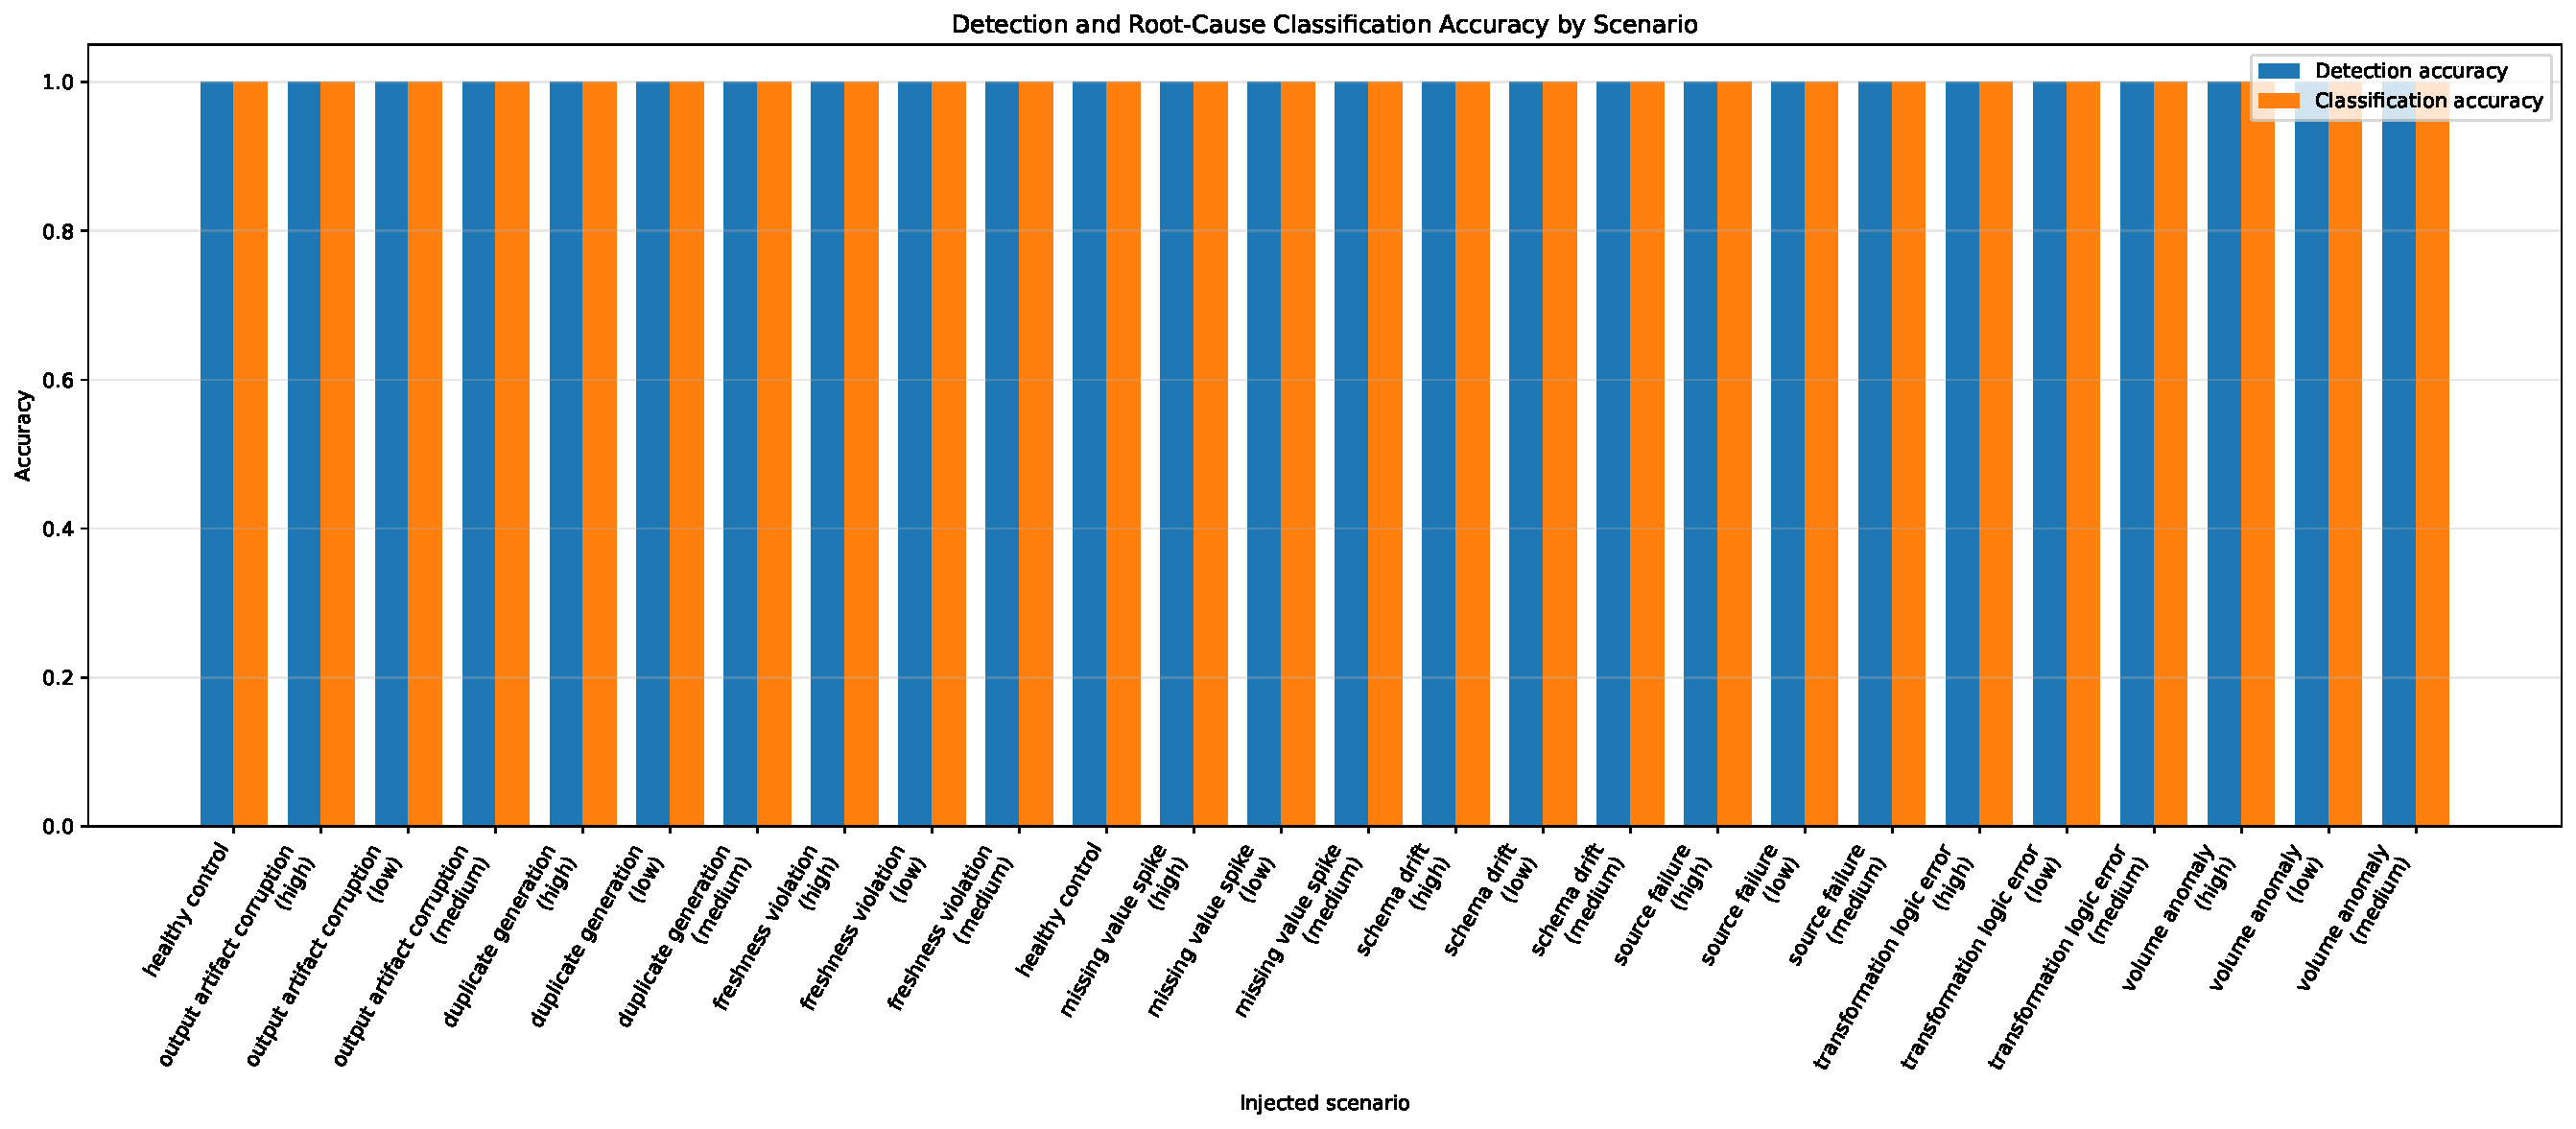
\includegraphics[width=\linewidth]{figures/figure_1_accuracy_by_scenario.pdf}
\caption{Detection and root-cause classification accuracy by injected scenario.}
\label{fig:accuracy-by-scenario}
\end{figure}

\begin{figure}[t]
\centering
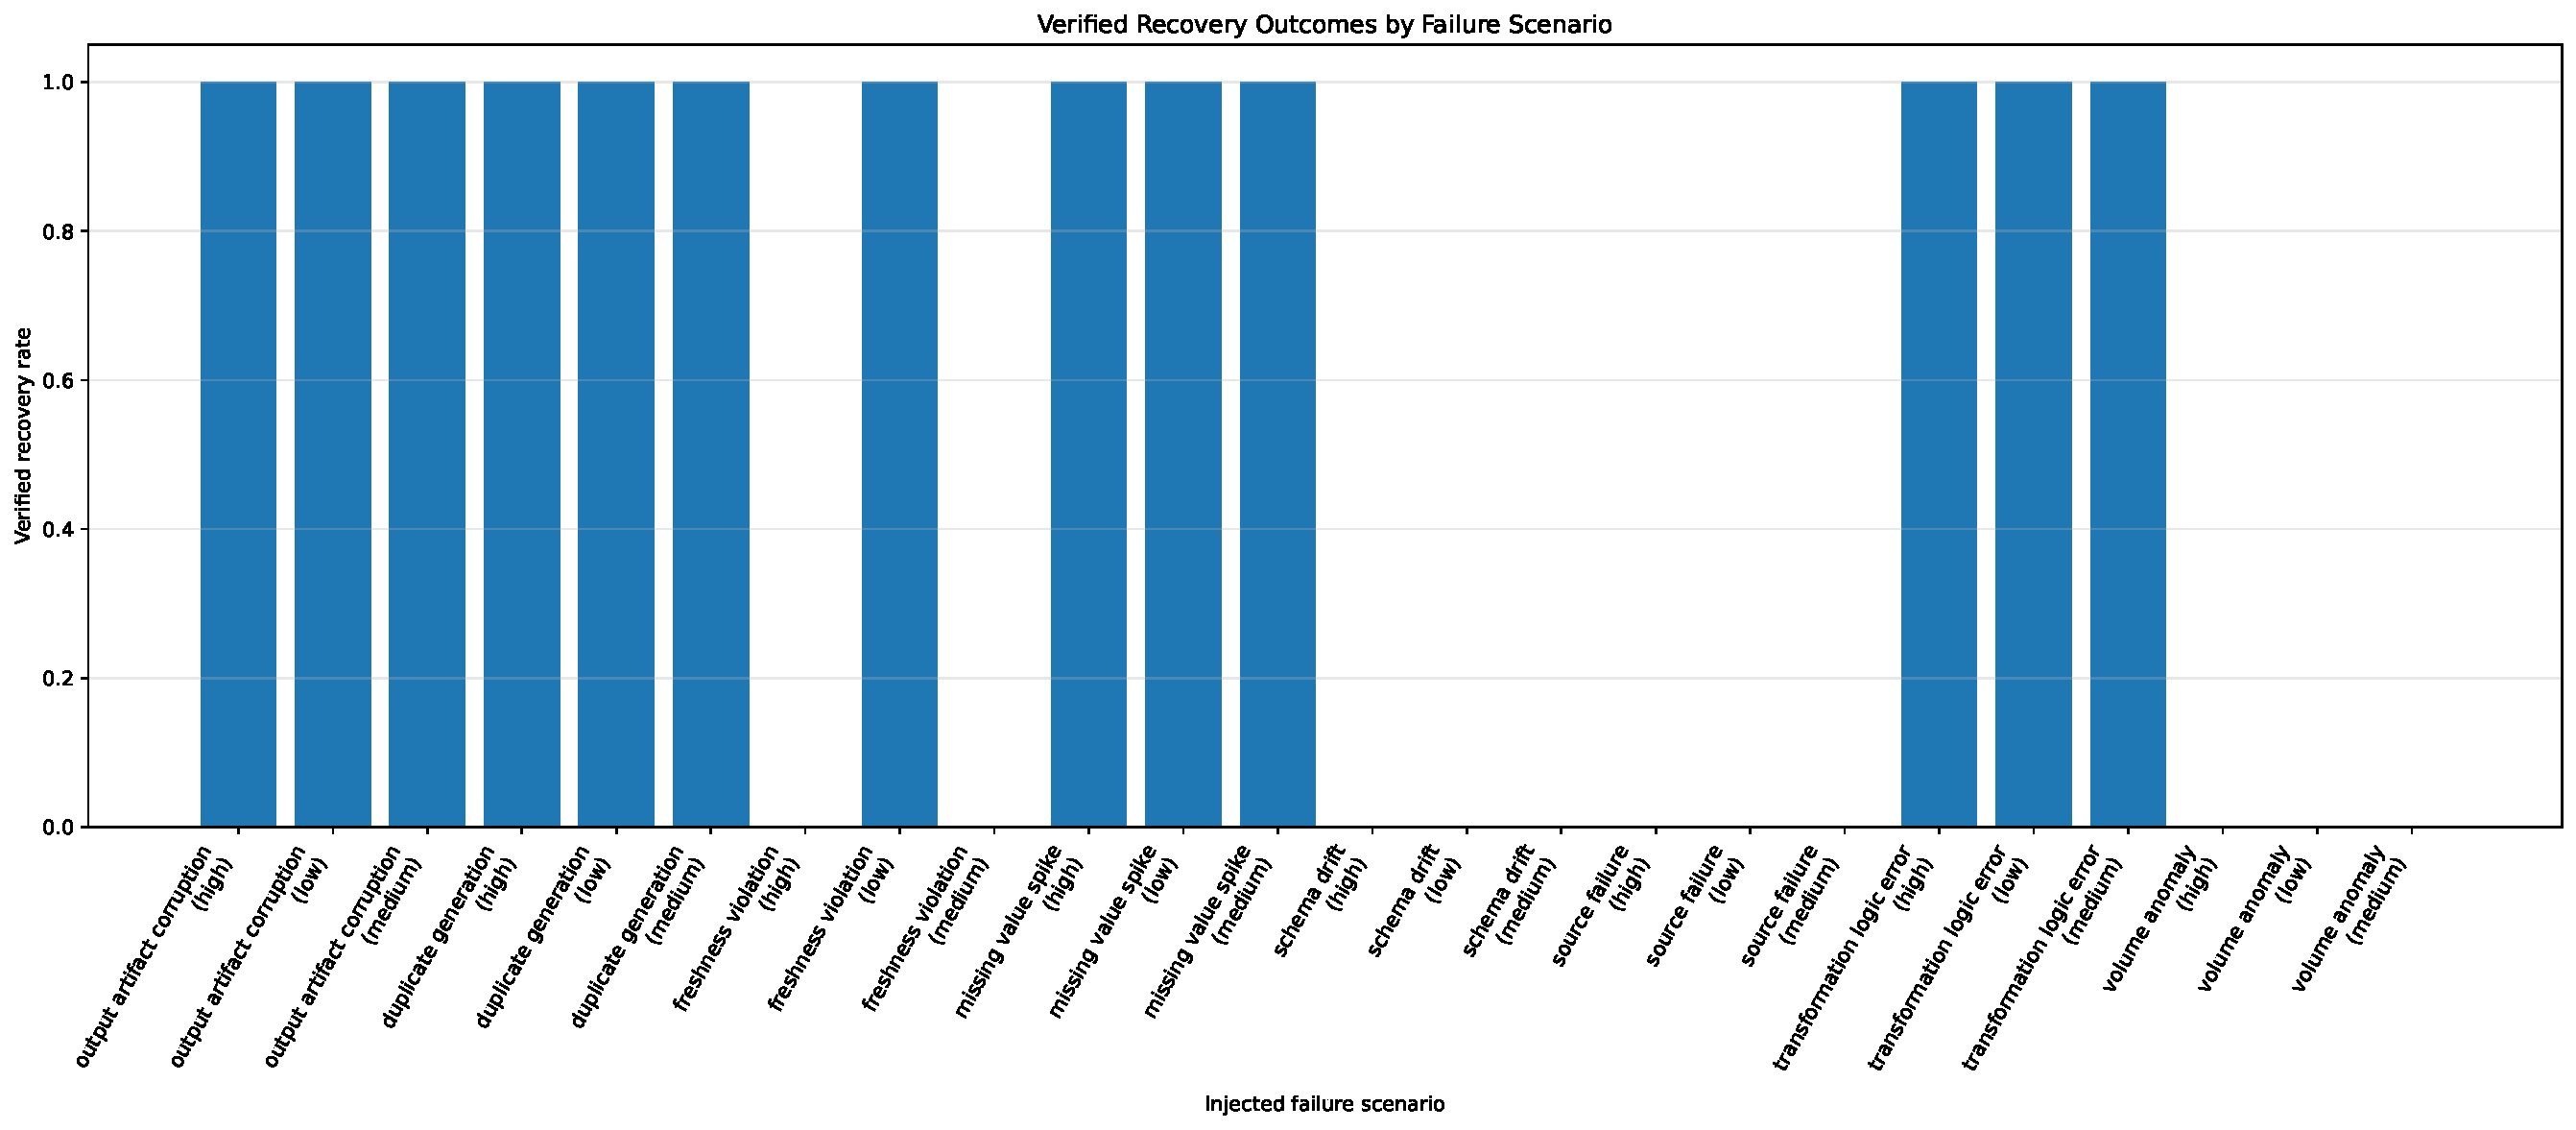
\includegraphics[width=\linewidth]{figures/figure_2_recovery_by_scenario.pdf}
\caption{Verified recovery outcomes by injected failure scenario.}
\label{fig:recovery-by-scenario}
\end{figure}

\begin{figure}[t]
\centering
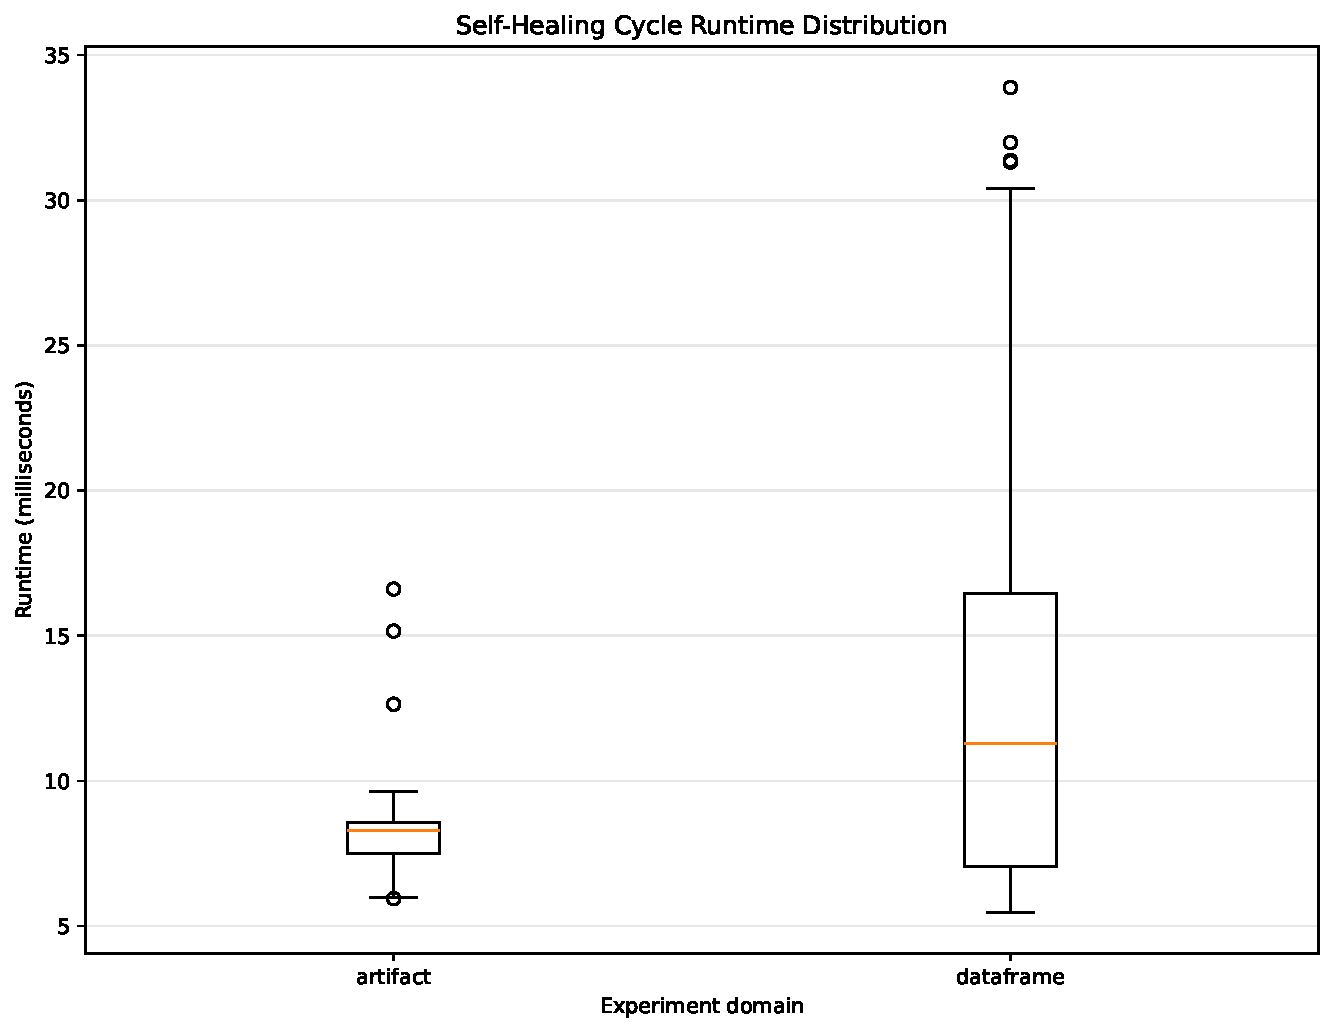
\includegraphics[width=\linewidth]{figures/figure_3_runtime_distribution.pdf}
\caption{Self-healing cycle runtime distribution.}
\label{fig:runtime-distribution}
\end{figure}

\begin{figure}[t]
\centering
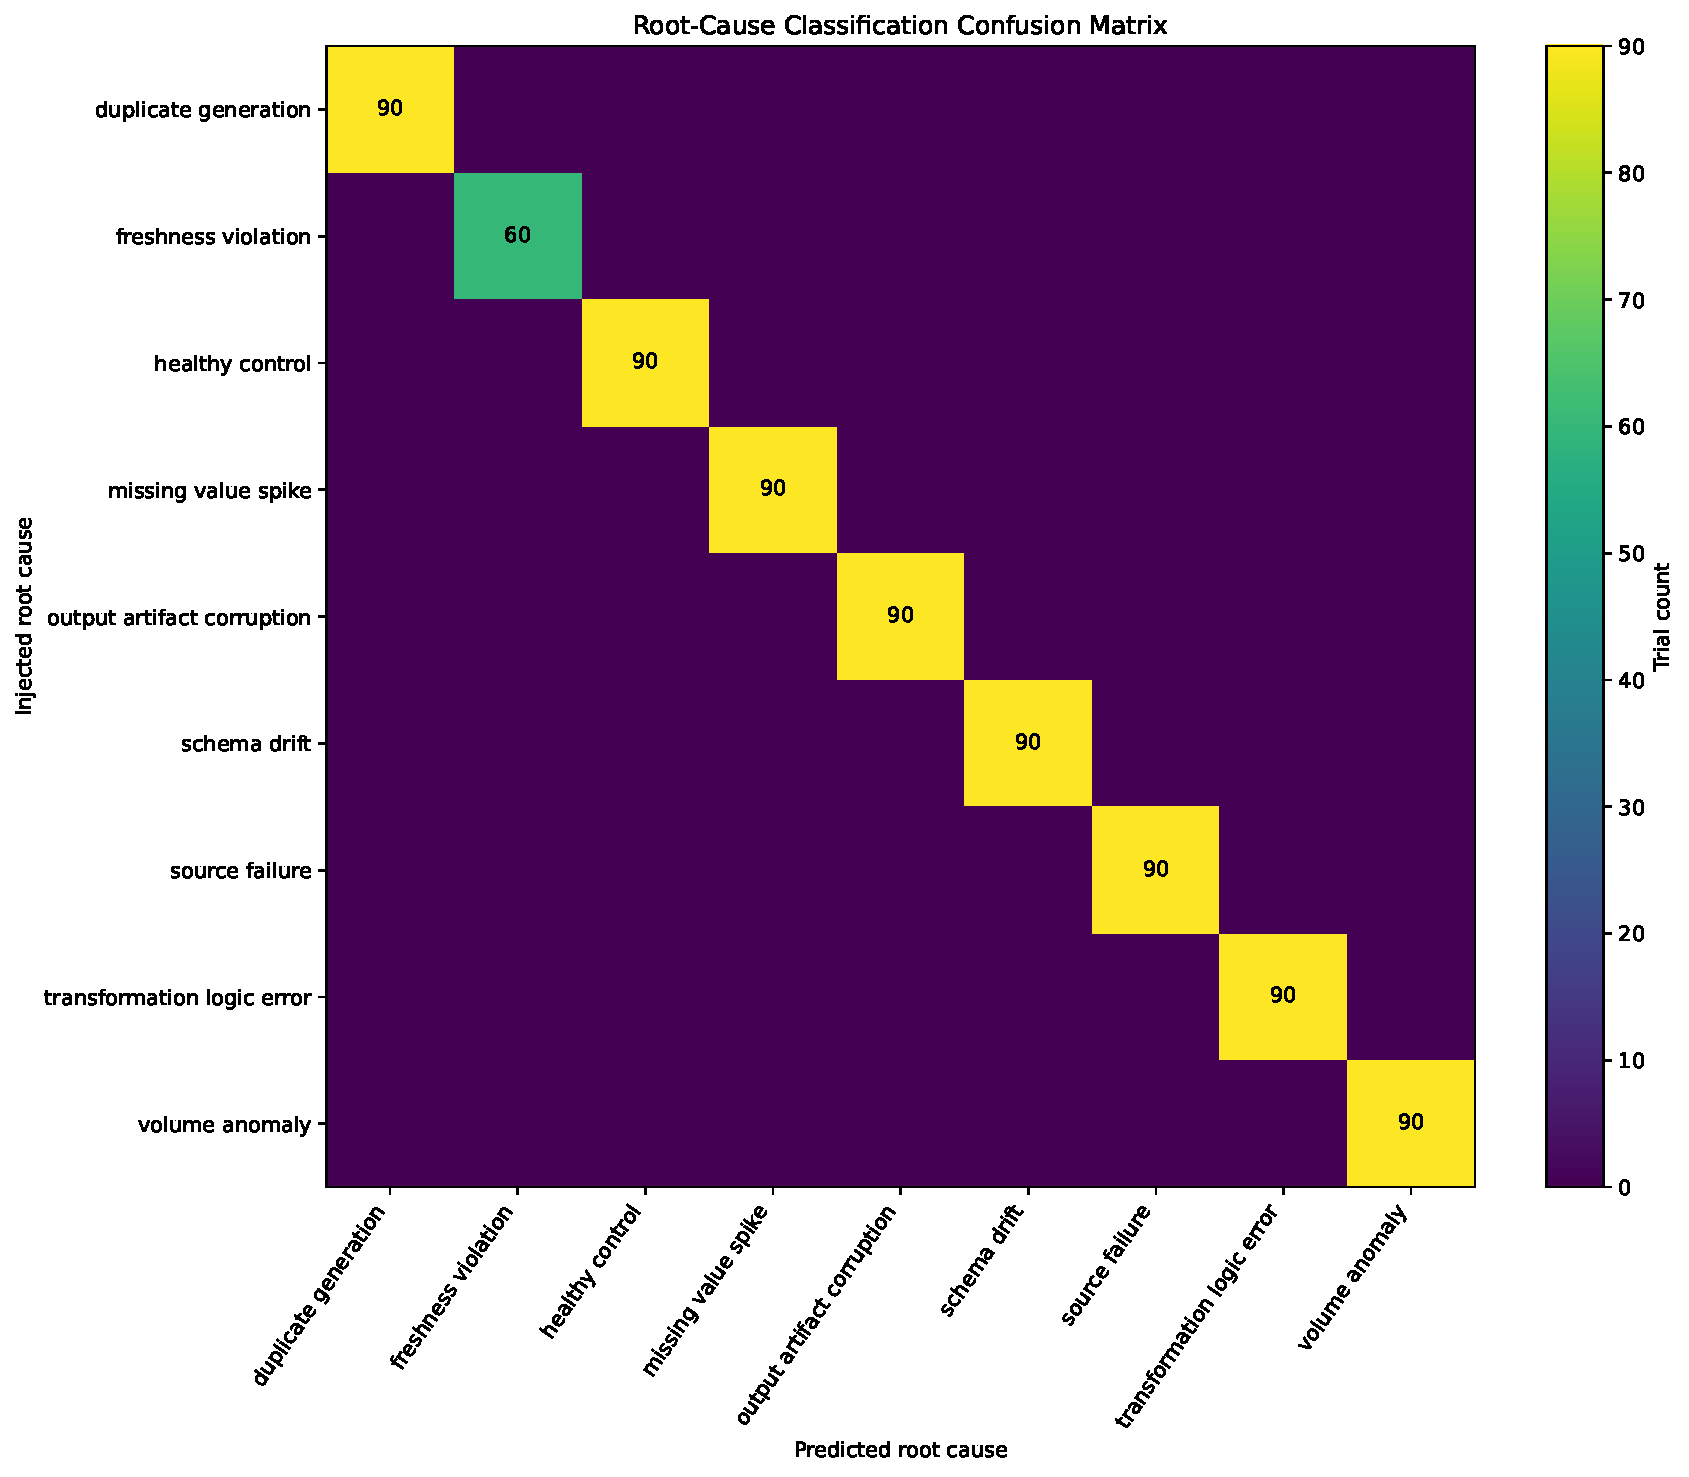
\includegraphics[width=\linewidth]{figures/figure_4_classification_confusion_matrix.pdf}
\caption{Root-cause classification confusion matrix.}
\label{fig:classification-confusion-matrix}
\end{figure}

